\documentclass[11pt,a4paper]{article}

\usepackage[margin=2.5cm]{geometry}
\usepackage[utf8]{inputenc}
\usepackage[T1]{fontenc}
\usepackage{booktabs}
\usepackage{array}
\usepackage{xcolor}
\usepackage{hyperref}
\usepackage{enumitem}
\usepackage{longtable}
\usepackage{tikz}
\usetikzlibrary{arrows.meta, positioning}

\hypersetup{
    colorlinks=true,
    linkcolor=blue!50!black,
    urlcolor=blue!50!black,
    pdftitle={CSI Motion Detection Project: File Inventory},
    pdfauthor={Ilyas}
}

\definecolor{pathgray}{RGB}{90,90,90}
\newcommand{\filepath}[1]{{\small\ttfamily\color{pathgray}#1}}

% One consistent template for every file entry.
\newcommand{\fileentry}[6]{%
    \subsection{\texttt{#1}}
    \filepath{#2}
    \vspace{0.15cm}
    \begin{description}[leftmargin=2.6cm, style=nextline]
        \item[Type] #3
        \item[Objective] #4
        \item[Role] #5
        \item[Connections] #6
    \end{description}
    \vspace{0.2cm}
    \hrule
    \vspace{0.3cm}
}

\title{\textbf{CSI Motion Detection Project}\\
\large Complete File Inventory: Name, Location, Objective, and Role of Every Non-Data File}
\author{Ilyas}
\date{\today}

\begin{document}

\maketitle
\tableofcontents
\newpage

\section{Scope of this document}

This document lists every file in the project that is code, configuration,
or a build artifact -- everything \emph{except} the raw recorded CSI
datasets (the \texttt{part\_1\_data} through \texttt{part\_5\_data}
folders and their CSVs). For each file it gives: what kind of file it is,
why it exists (the specific problem it was written to solve), what it
concretely does, and how it connects to the other files in the pipeline.

Files are grouped into four categories, matching the four phases of the
project: firmware, data collection and verification, model training and
validation, and live inference.

% =====================================================================
\section{Firmware and Build Configuration}
% =====================================================================

These files run on the ESP32-S3 itself, or configure how it is built and
flashed. They are the only files in the project that do not run on the
host PC.

\fileentry
{main/csi\_node.c}
{csi\_node/main/csi\_node.c}
{C source (ESP-IDF component), 247 lines}
{Capture Wi-Fi Channel State Information from the device's live
    connection to the router, at a steady frame rate, and stream it over
    USB serial in a format the host-side Python tooling can parse.}
{Connects to Wi-Fi in station mode; captures the associated access
    point's BSSID so CSI from other nearby devices can be filtered out;
    runs a background 100\,ms-interval ping to the router to trigger a
    steady \(\approx\)10\,Hz stream of CSI updates; enables the ESP32's
    CSI extraction API; and prints each frame as a single
    \texttt{CSI\_AMP,\ldots} line over UART. Internally, the CSI callback
    only copies data into a queue (it does no formatting or I/O itself),
    and a separate, lower-priority task drains that queue and does the
    actual amplitude computation and printing -- this split exists
    specifically because an earlier, simpler version that did this work
    directly in the callback stalled the Wi-Fi radio and halved the
    frame rate. A small serial-input task also lets a terminal manually
    set the current label (\texttt{e}/\texttt{s}/\texttt{m}) as a
    fallback to the host-driven labeling used during normal collection.}
{This is the root of the entire pipeline: every other file in the
    project either produces data derived from this firmware's output, or
    consumes its live serial stream directly. Read by
    \texttt{csi\_label\_collector.py}, \texttt{csi\_live\_monitor.py},
    \texttt{csi\_live\_predict.py}, and \texttt{csi\_live\_server.py}.}

\fileentry
{main/CMakeLists.txt}
{csi\_node/main/CMakeLists.txt}
{ESP-IDF component build file}
{Tell the ESP-IDF build system which source files make up the
    \texttt{main} component and where its headers live.}
{A two-line standard ESP-IDF component manifest:
    \texttt{idf\_component\_register(SRCS "csi\_node.c" INCLUDE\_DIRS ".")}.
    It does not contain any project-specific logic.}
{Required by the ESP-IDF build system whenever \texttt{main/csi\_node.c}
    is compiled or flashed; not read by anything on the host side.}

\fileentry
{CMakeLists.txt}
{csi\_node/CMakeLists.txt}
{ESP-IDF top-level project build file}
{Declare \texttt{csi\_node} as an ESP-IDF project and pull in the
    standard ESP-IDF project build rules.}
{Boilerplate: sets the minimum CMake version, includes ESP-IDF's
    \texttt{project.cmake}, and names the project. Unmodified from the
    ESP-IDF project template.}
{Root of the CMake build graph; everything under \texttt{main/} and the
    generated \texttt{build/} directory descends from this file. Not
    used by any Python tooling.}

\fileentry
{sdkconfig}
{csi\_node/sdkconfig}
{ESP-IDF generated project configuration}
{Record every board- and project-level configuration choice (Wi-Fi
    buffers, partition table, and critically, the UART/USB-serial
    console baud rate) so builds are reproducible.}
{Machine-generated and machine-maintained by \texttt{idf.py menuconfig};
    not hand-authored. The one setting that matters most for the rest of
    this project is
    \texttt{CONFIG\_ESP\_CONSOLE\_UART\_BAUDRATE=115200}, which is why
    every host-side script that opens the serial port
    (\texttt{csi\_label\_collector.py}, \texttt{csi\_live\_monitor.py},
    \texttt{csi\_live\_predict.py}, \texttt{csi\_live\_server.py}) must be
    run with \texttt{-b 115200} to actually receive readable data.}
{Consulted only indirectly: every serial-opening script's baud-rate
    argument must match the value stored here.}

% =====================================================================
\section{Data Collection and Verification}
% =====================================================================

These two files run on the host PC \emph{during} a recording session,
before any model exists. They turn the firmware's live serial stream
into either a labeled dataset or a human-readable visual check.

\fileentry
{csi\_label\_collector.py}
{Codex/2026-07-21/wh/outputs/csi\_label\_collector.py}
{Python script (host-side), \(\approx\)280 lines}
{Turn the firmware's raw serial stream into a labeled, quality-checked
    CSV dataset, while solving a specific labeling problem: recording
    ``empty'' requires the operator to be physically absent, and
    recording ``moving'' requires them to be present, so the two labels
    cannot both be triggered by the same person in the room at the same
    time.}
{Drives an explicit state machine per recording cycle: a 5-second
    \texttt{LEAVE} countdown (frames tagged \texttt{settling=1} and
    later excluded from training), then a 60-second automatic
    \texttt{EMPTY} recording (label 0), then a \texttt{WAIT} state until
    the operator presses \texttt{m} upon returning, then a 60-second
    \texttt{MOVING} recording (label 2) -- and repeats. It parses each
    incoming \texttt{CSI\_AMP} line, locks onto the first
    session's subcarrier count and \textbf{rejects} (rather than pads)
    any frame whose count later disagrees -- the direct fix for an
    earlier bug where a mid-recording Wi-Fi bandwidth change silently
    mixed 128- and 192-subcarrier frames in the same file. It writes
    both a combined \texttt{all\_csi\_data.csv} and a per-label CSV per
    session folder.}
{Consumes the live serial stream from \texttt{main/csi\_node.c} directly
    (one process, exclusive access to the COM port). Produces the
    \texttt{part\_N\_data/} folders that \texttt{train\_model.py},
    \texttt{evaluate\_holdout.py}, and \texttt{analyze\_model.py} all
    read. Shares its line-format parsing logic conceptually with
    \texttt{csi\_common.py}, though it predates that shared module and
    still contains its own copy.}

\fileentry
{csi\_live\_monitor.py}
{Codex/2026-07-21/wh/outputs/csi\_live\_monitor.py}
{Python script (host-side, Matplotlib), \(\approx\)220 lines}
{Give a human a fast visual way to confirm the CSI channel is actually
    reacting to a person moving in and out of the room, \emph{before}
    committing to a full labeled recording session -- and to do so
    smoothly enough to be trustworthy as a live check, not distractingly
    laggy.}
{Reads the live serial stream and renders a scrolling waterfall
    (subcarrier amplitude over time) plus a frame-to-frame motion-energy
    line, using a fixed color scale calibrated once from the first
    \(\sim\)30 frames rather than recomputed every frame (recomputing
    every frame was found to cause both lag and visible flicker). Prints
    a simple ``MOTION DETECTED'' / ``quiet / empty'' status text driven
    by a fixed-threshold heuristic on the motion-energy trace -- this
    predates the trained model and is not the same thing as a model
    prediction.}
{Reads the same live serial stream as \texttt{csi\_label\_collector.py}
    (cannot run at the same time as it -- only one process may hold the
    COM port). Conceptually the direct ancestor of
    \texttt{csi\_live\_predict.py}, which extends this same
    waterfall/energy visualization with an actual trained-model
    prediction in place of the fixed-threshold heuristic.}

% =====================================================================
\section{Model Training and Validation}
% =====================================================================

These files never touch the serial port. They run entirely offline,
against already-recorded CSV data, and produce (or evaluate) the trained
model.

\fileentry
{csi\_common.py}
{csi\_node/csi\_common.py}
{Python module (shared library), \(\approx\)130 lines}
{Have exactly one implementation of the CSI line-parsing and
    feature-extraction math, shared by every training script and every
    live-inference script -- so the offline (training) and online
    (live) code paths can never silently diverge from each other, which
    would otherwise be a very easy and very hard-to-notice bug.}
{Provides: \texttt{parse\_line} (turns a raw \texttt{CSI\_AMP,\ldots}
    line into an RSSI value and an amplitude array);
    \texttt{raw\_window\_stats} (per-window mean/std of amplitude,
    motion energy, and RSSI); \texttt{compute\_baseline} and
    \texttt{calibrate\_features} (turn raw stats into baseline-relative
    features -- amplitude/RSSI means become deltas, standard deviations
    become ratios against a calibration baseline, which is what makes
    the model robust to a session's absolute noise floor having drifted
    since training); \texttt{feature\_names} (the canonical, ordered
    list of feature names, so every consumer agrees on feature order);
    and \texttt{PredictionSmoother} (majority-vote hysteresis over the
    last 5 raw window predictions, so a single noisy window cannot flip
    the displayed live state).}
{Imported by \texttt{train\_model.py}, \texttt{evaluate\_holdout.py},
    \texttt{analyze\_model.py}, \texttt{csi\_live\_predict.py}, and
    \texttt{csi\_live\_server.py}. This is the single most
    architecturally important file in the project: every other Python
    file that touches features, calibration, or smoothing goes through
    this module rather than reimplementing the math.}

\fileentry
{train\_model.py}
{csi\_node/train\_model.py}
{Python script (offline training), \(\approx\)175 lines}
{Turn a set of labeled recording sessions into a trained, validated
    Random Forest classifier, and produce an honest estimate of how well
    it generalizes to a session it has not seen.}
{For each named session folder: loads the CSV, drops the
    \texttt{settling=1} transition frames, computes that session's
    calibration baseline from the first 10 seconds of its first
    confirmed-empty block, and splits the remainder into fixed
    2-second windows (discarding any window that spans a label change).
    Each window becomes one calibrated feature vector via
    \texttt{csi\_common.calibrate\_features}. It then runs
    leave-one-session-out cross-validation
    (\texttt{sklearn.model\_selection.LeaveOneGroupOut}, one fold per
    session) to report a realistic accuracy estimate, refits a final
    \texttt{RandomForestClassifier} on all sessions combined, and saves
    it -- together with the subcarrier columns, feature names, window
    size, calibration duration, and frame rate it was trained with -- to
    \texttt{csi\_model.joblib}.}
{Reads the \texttt{part\_N\_data/} folders produced by
    \texttt{csi\_label\_collector.py}. Uses
    \texttt{csi\_common.compute\_baseline}, \texttt{calibrate\_features},
    and \texttt{feature\_names}. Its \texttt{build\_dataset} function is
    imported directly by both \texttt{evaluate\_holdout.py} and
    \texttt{analyze\_model.py}, so all three scripts window and
    calibrate data identically. Its output,
    \texttt{csi\_model.joblib}, is the single artifact that
    \texttt{csi\_live\_predict.py} and \texttt{csi\_live\_server.py}
    load to make live predictions.}

\fileentry
{evaluate\_holdout.py}
{csi\_node/evaluate\_holdout.py}
{Python script (offline validation), \(\approx\)55 lines}
{Answer a stricter question than leave-one-session-out can: does the
    model generalize to a session that never contributed to training at
    all, in any fold -- the check that actually caught two contaminated
    or environment-shifted recordings before they could reach the
    training pool.}
{Takes an explicit list of training sessions and an explicit list of
    test sessions (disjoint), builds calibrated feature sets for each
    using \texttt{train\_model.build\_dataset}, fits a
    \texttt{RandomForestClassifier} on the training sessions only, and
    reports accuracy, a full classification report, and a confusion
    matrix on the test session(s). Used as the gate every new session in
    this project has been run through before being folded into the
    permanent training pool.}
{Imports \texttt{build\_dataset} from \texttt{train\_model.py}, and
    therefore transitively depends on \texttt{csi\_common.py} for all
    feature math. Reads whichever \texttt{part\_N\_data/} folders are
    passed on the command line; does not write any files itself
    (diagnostic-only).}

\fileentry
{analyze\_model.py}
{csi\_node/analyze\_model.py}
{Python script (offline reporting), \(\approx\)90 lines}
{Extract every number needed to visually explain how well the model
    performs -- per-fold accuracy, confusion matrices, feature
    importances, class balance, and the motion-energy distributions that
    separate the two classes -- without hand-copying numbers out of
    training logs.}
{Re-runs the same leave-one-session-out pipeline as
    \texttt{train\_model.py} (via the same \texttt{build\_dataset}
    function), but additionally extracts the fitted model's
    \texttt{feature\_importances\_}, the per-class motion-energy values
    for every window, and per-session class counts, and writes all of it
    to \texttt{model\_analysis.json} as a single structured file.}
{Imports \texttt{build\_dataset} from \texttt{train\_model.py} and
    \texttt{feature\_names} from \texttt{csi\_common.py}. Its JSON
    output was consumed by a standalone HTML/JavaScript training-report
    dashboard built earlier in the project (charts of per-fold accuracy,
    confusion matrices, feature importance, and the motion-energy
    histogram) -- a one-off visualization artifact, not part of the
    ongoing pipeline.}

\fileentry
{csi\_model.joblib}
{csi\_node/csi\_model.joblib}
{Binary artifact (joblib-serialized Python object), not source code}
{Persist the trained classifier together with everything needed to
    reproduce its exact feature pipeline at inference time, so training
    and live inference can never silently drift apart (e.g.\ a different
    window size or calibration duration being assumed on each side).}
{A dictionary containing: the fitted \texttt{RandomForestClassifier}
    itself; the ordered list of amplitude column names (subcarrier
    count and order); the ordered feature names; the window size in
    seconds; the calibration duration in seconds; and the frame rate.
    Regenerated every time \texttt{train\_model.py} is run.}
{Produced by \texttt{train\_model.py}. Loaded by
    \texttt{csi\_live\_predict.py} and \texttt{csi\_live\_server.py} at
    startup -- both read its stored window size, calibration duration,
    and frame rate rather than hardcoding them, so retraining with
    different settings automatically propagates to live inference.}

% =====================================================================
\section{Live Inference}
% =====================================================================

These files run the trained model against the firmware's live serial
stream in real time, as two independent front ends sharing the same
underlying logic.

\fileentry
{csi\_live\_predict.py}
{csi\_node/csi\_live\_predict.py}
{Python script (host-side, Matplotlib), \(\approx\)250 lines}
{Provide a real-time, on-screen empty/moving prediction using the actual
    trained model, in the same waterfall-plot format already familiar
    from \texttt{csi\_live\_monitor.py} -- a single desktop window, no
    browser or extra process required.}
{Loads \texttt{csi\_model.joblib} and reads its calibration duration and
    window size. On startup, buffers the first calibration period of
    incoming frames (during which the operator must leave the room) and
    computes a baseline via \texttt{csi\_common.compute\_baseline}.
    After that, every new frame recomputes calibrated features for the
    current rolling window via \texttt{csi\_common.make\_features} and
    predicts; the raw per-window prediction is passed through a
    \texttt{csi\_common.PredictionSmoother} before being displayed, so
    the on-screen status only changes once a majority of the last 5
    windows agree. Displays ``CALIBRATING'', ``warming up'', or the
    smoothed \texttt{EMPTY}/\texttt{MOVING} state with confidence, color
    coded, above the same waterfall and motion-energy plot as the
    original monitor.}
{Reads the live serial stream from \texttt{main/csi\_node.c}. Loads
    \texttt{csi\_model.joblib} (produced by \texttt{train\_model.py}) and
    uses \texttt{csi\_common.py} for parsing, calibration, feature
    extraction, and smoothing -- identical math to
    \texttt{csi\_live\_server.py}, just a different display layer.}

\noindent\textit{\texttt{csi\_live\_predict.py} uses \texttt{csi\_common.py} for all
parsing, calibration, and smoothing logic -- see its entry in
Section~3 (Model Training and Validation) for details.}

\vspace{0.3cm}

\fileentry
{csi\_live\_server.py}
{csi\_node/csi\_live\_server.py}
{Python script (host-side backend), \(\approx\)235 lines}
{Make the same live prediction available to a browser-based UI, since a
    browser cannot open a Windows COM port directly (short of the
    Chrome-only Web Serial API, which would additionally require
    re-implementing the trained Random Forest's decision logic in
    JavaScript -- a source of risk that was deliberately avoided).}
{Opens the serial port in a background thread and parses incoming
    frames, logging periodic byte/line/parsed-frame counts and echoing
    unrecognized lines to the console for diagnosability (added after an
    earlier version silently hung with no visible cause when the serial
    link produced no data). Runs the same calibration-then-predict-
    then-smooth pipeline as \texttt{csi\_live\_predict.py}, using the
    same \texttt{csi\_common.py} functions, but instead of drawing a
    plot itself, broadcasts every result as a JSON message over a local
    WebSocket server (\texttt{ws://localhost:8765}) to any connected
    browser tab. Caches the most recent status message of each type
    (error, warning, calibration state) and replays it to any client
    that connects after that message was first sent, so a client that
    opens the dashboard late still learns what happened.}
{Reads the live serial stream from \texttt{main/csi\_node.c}. Loads
    \texttt{csi\_model.joblib} and uses \texttt{csi\_common.py}
    identically to \texttt{csi\_live\_predict.py}. Its sole consumer is
    \texttt{csi\_dashboard.html}, connecting over WebSocket.}

\fileentry
{csi\_dashboard.html}
{csi\_node/csi\_dashboard.html}
{Self-contained HTML/CSS/JavaScript page, \(\approx\)400 lines}
{Give the live prediction a cleaner, more customizable visual
    presentation than Matplotlib allows, run as an ordinary local web
    page rather than a desktop application window.}
{A single static file with no build step and no server framework
    dependency: opening it directly in a browser is sufficient. It
    connects to \texttt{csi\_live\_server.py}'s WebSocket, renders the
    waterfall as a scrolling \texttt{canvas} heatmap (pixel-level
    control, resized via CSS rather than redrawn from scratch every
    frame for performance), draws the motion-energy trace as an SVG
    sparkline, and shows a large color-coded status badge (green
    \texttt{EMPTY}, red \texttt{MOVING}, amber \texttt{CALIBRATING}) with
    both the smoothed/confirmed prediction and the raw current-window
    prediction visible. Automatically reconnects if the WebSocket drops,
    and supports both light and dark themes.}
{Its only data source is \texttt{csi\_live\_server.py}, over
    \texttt{ws://localhost:8765}; it contains no Python and does not
    read any file on disk directly.}

% =====================================================================
\section{File Relationship Diagram}
% =====================================================================

Figure~\ref{fig:filegraph} summarizes the dependency relationships
described above: which files read, import, or are produced by which
others.

\begin{figure}[h]
\centering
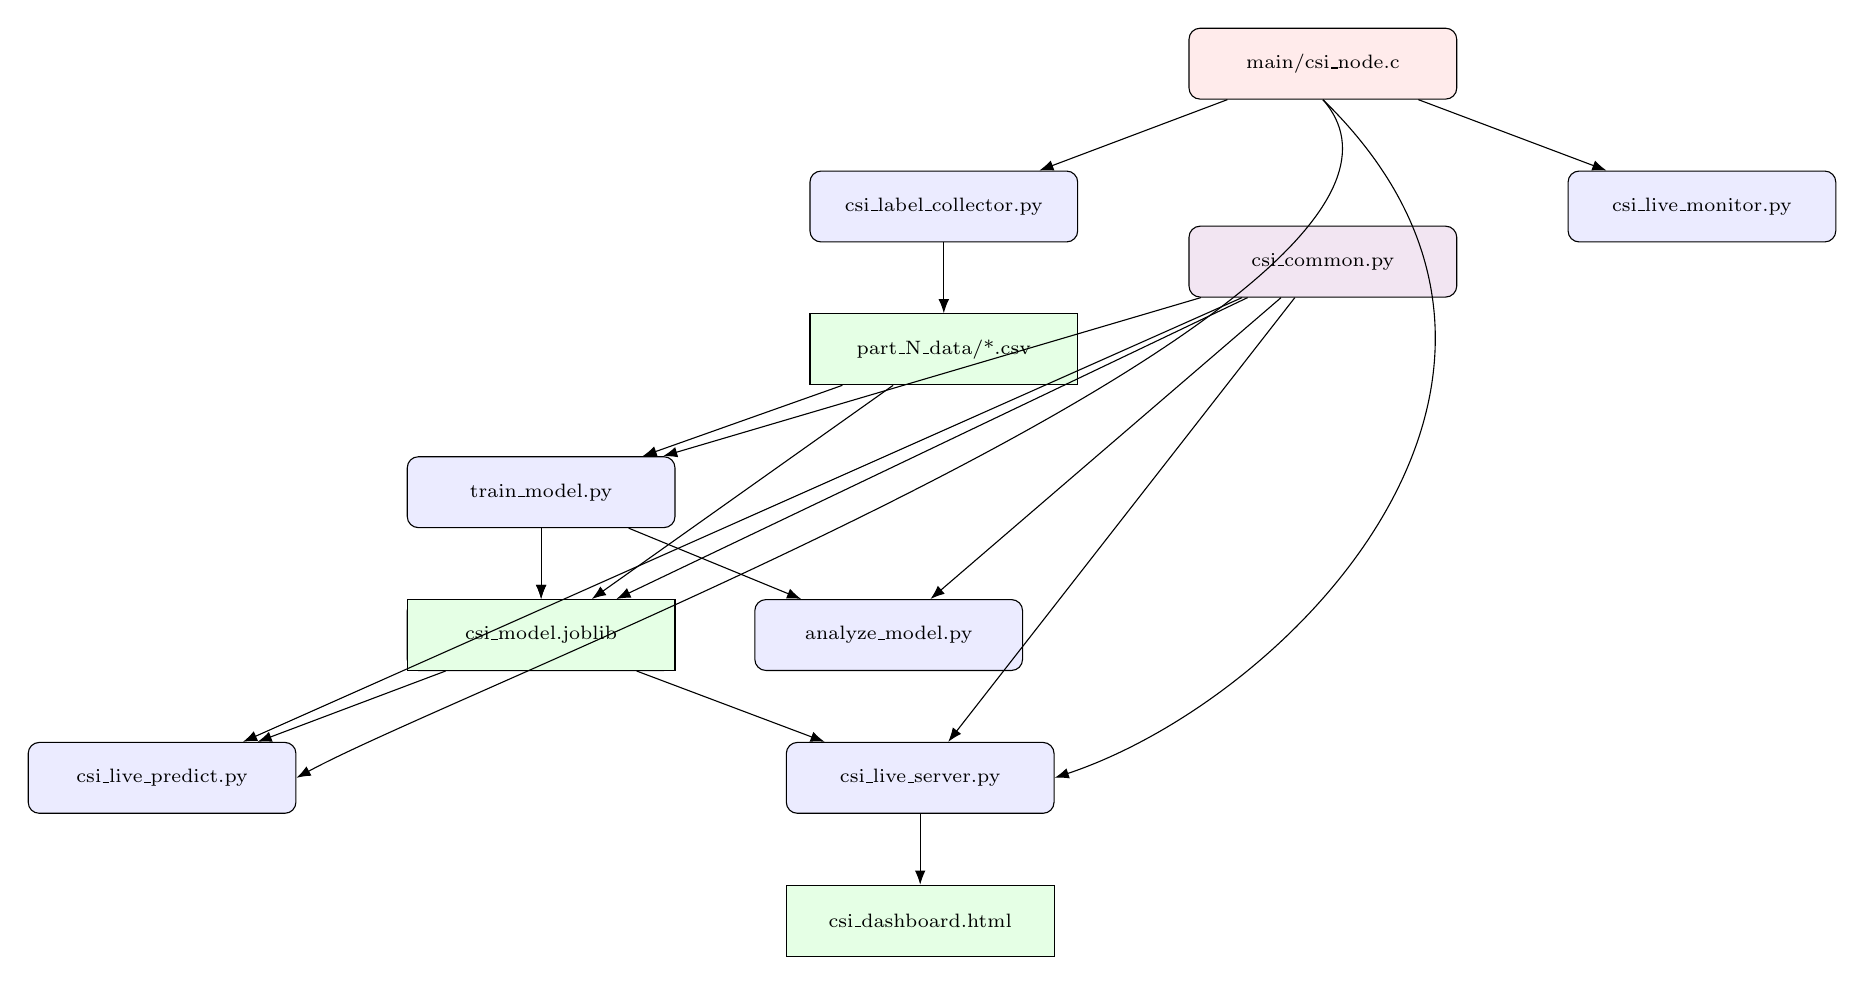
\begin{tikzpicture}[
    node distance=0.9cm and 1.4cm,
    fw/.style={draw, rounded corners, minimum width=3.4cm, minimum height=0.9cm, align=center, font=\scriptsize, fill=red!8},
    host/.style={draw, rounded corners, minimum width=3.4cm, minimum height=0.9cm, align=center, font=\scriptsize, fill=blue!8},
    lib/.style={draw, rounded corners, minimum width=3.4cm, minimum height=0.9cm, align=center, font=\scriptsize, fill=violet!10},
    art/.style={draw, minimum width=3.4cm, minimum height=0.9cm, align=center, font=\scriptsize, fill=green!10},
    arrow/.style={-{Latex[length=1.8mm]}, thin}
]
    \node[fw] (fw) {main/csi\_node.c};
    \node[host, below left=of fw] (coll) {csi\_label\_collector.py};
    \node[host, below right=of fw] (mon) {csi\_live\_monitor.py};
    \node[art, below=of coll] (csv) {part\_N\_data/*.csv};
    \node[lib, below=1.6cm of fw] (common) {csi\_common.py};
    \node[host, below left=of csv, xshift=-0.3cm] (train) {train\_model.py};
    \node[host, below=of train] (holdout) {evaluate\_holdout.py};
    \node[host, right=1.0cm of holdout] (analyze) {analyze\_model.py};
    \node[art, below=of train] (model) {csi\_model.joblib};
    \node[host, below left=of model] (predict) {csi\_live\_predict.py};
    \node[host, below right=of model] (server) {csi\_live\_server.py};
    \node[art, below=of server] (dash) {csi\_dashboard.html};

    \draw[arrow] (fw) -- (coll);
    \draw[arrow] (fw) -- (mon);
    \draw[arrow] (coll) -- (csv);
    \draw[arrow] (csv) -- (train);
    \draw[arrow] (csv) -- (holdout);
    \draw[arrow] (common) -- (train);
    \draw[arrow] (common) -- (holdout);
    \draw[arrow] (common) -- (analyze);
    \draw[arrow] (common) -- (predict);
    \draw[arrow] (common) -- (server);
    \draw[arrow] (train) -- (holdout);
    \draw[arrow] (train) -- (analyze);
    \draw[arrow] (train) -- (model);
    \draw[arrow] (model) -- (predict);
    \draw[arrow] (model) -- (server);
    \draw[arrow] (server) -- (dash);
    \draw[arrow] (fw.south) .. controls +(2.2,-2.5) and +(2.2,1.2) .. (predict.east);
    \draw[arrow] (fw.south) .. controls +(3.6,-3.5) and +(3.0,1.0) .. (server.east);
\end{tikzpicture}
\caption{File relationships. Red: firmware. Blue: host-side scripts. Violet: shared library. Green: data/model artifacts. Long curved arrows show the two live-inference scripts also reading the firmware's serial stream directly.}
\label{fig:filegraph}
\end{figure}

\end{document}
